\documentclass[12pt, openany]{report}
\usepackage[utf8]{inputenc}
\usepackage[T1]{fontenc}
\usepackage{amsmath,amsfonts,amssymb}
\usepackage{amssymb}
\usepackage{multicol}
\usepackage[a4paper,left=2.5cm,right=2.5cm,top=2.5cm,bottom=2.5cm]{geometry}
\usepackage[english]{babel}
\usepackage{libertine}
\usepackage{graphicx}
\usepackage{wrapfig}
\usepackage{algorithm}
\usepackage{algpseudocode}
\usepackage{float}
\usepackage{enumitem}
\usepackage{pythonhighlight}
\usepackage[]{titletoc}
\usepackage{empheq}
\usepackage{titlesec}
\usepackage{mathpazo}
\usepackage{xfrac}
\usepackage{textcomp}
\usepackage{mathtools}
\usepackage{caption}
\usepackage{tabularray}
\usepackage{subcaption}
\usepackage[bottom]{footmisc}
\usepackage{pdfpages}
\usepackage{tabularx}
\usepackage{amsthm}
\usepackage{listings}
\usepackage[skins]{tcolorbox}
\titleformat{\chapter}[display]
  {\normalfont\bfseries}{}{0pt}{\Huge}
\usepackage{hyperref}
\newcommand{\hsp}{\hspace{20pt}}
\newcommand{\HRule}{\rule{\linewidth}{0.5mm}}
\newcommand{\R}{\mathbb{R}}
\newcommand{\C}{\mathbb{C}}
\theoremstyle{definition}
\newtheorem{thm}{Theorem}[chapter]
\newtheorem{definition}[thm]{Definition}
\newtheorem{lem}[thm]{Lemma}


\definecolor{mGreen}{rgb}{0,0.6,0}
\definecolor{mGray}{rgb}{0.5,0.5,0.5}
\definecolor{mPurple}{rgb}{0.58,0,0.82}
\definecolor{backgroundColour}{rgb}{0.95,0.95,0.92}
\definecolor{light-gray}{gray}{0.95}
\newcommand{\code}[1]{\colorbox{light-gray}{\texttt{#1}}}

\lstdefinestyle{CppStyle}{
    backgroundcolor=\color{backgroundColour},   
    commentstyle=\color{mGreen},
    keywordstyle=\color{magenta},
    numberstyle=\tiny\color{mGray},
    stringstyle=\color{mPurple},
    basicstyle=\footnotesize,
    breakatwhitespace=false,         
    breaklines=true,                 
    captionpos=b,                    
    keepspaces=true,                 
    numbers=left,                    
    numbersep=5pt,                  
    showspaces=false,                
    showstringspaces=false,
    showtabs=false,                  
    tabsize=2,
    language=C
}

\hbadness=100000
\begin{document}
\begin{titlepage}
    \begin{sffamily}
    \begin{center}
        
\includegraphics[scale=0.3]{img/page_de_garde.png} \\[1cm]
        \HRule \\[0.4cm]
        { \huge \bfseries LINFO2365 Constraint Programming \\[0.4cm] }
    
        \HRule \\[1.5cm]
        \textsc{\LARGE Issambre L'Hermite Dumont}\\[3cm]
        {This summary may not be up-to-date, the newer version is available at this address: \hyperlink{https://github.com/SimonDesmidt/Syntheses}{https://github.com/SimonDesmidt/Syntheses}}
        \vfill
        \vspace{2cm}
        {\large Academic year 2025-2026 - Q2}
        \vspace{0.4cm}
         
        
\includegraphics[width=0.15\textwidth]{img/epl.png}
        
        UCLouvain\\
    
    \end{center}
    \end{sffamily}
\end{titlepage}

\setcounter{tocdepth}{1}
\tableofcontents
\chapter{Introduction}
Constraint programming (CP) is a paradigm for solving combinatorial problems and especially satisfaction problems. It is a complete method, given enough time, for satisfaction problems it can either prove that no solution exists or find a or all solution and for an optimization problem it can find an optimal solution if one exists. It is based on the idea of modeling a problem as a set of variables, each with a domain of possible values, and a set of constraints that specify the relationships between the variables. The goal is then to find an assignment of values to the variables that satisfies all the constraints. Additionnally to the satisfaction problems, we can also do optimization problems with CP by minimizing or maximizing some objective function. Constraint programming allows us to implement complex constraints very intuitively, this allows us to solve problems that are difficult to solve with other methods. Constraint programming is widely used in various fields such as scheduling, planning, resource allocation, and combinatorial optimization.\\
Constraint programming is a subfield of declarative programming, which is a programming paradigm that focuses on describing what the program should accomplish rather than how to accomplish it. So in our case, we will use constraint programming to describe the properties of the solution we are looking for, and the constraint solver will take care of finding a solution that satisfies those properties.\\
A constraint programming program consists of 2 main parts: the model and the search. The model is where we define the variables (e.g. $x$, $y$), their domains (e.g. $D_x = D_y = \{0,1\}$), and the constraints (e.g. $x \neq y$). The search is where we define the strategy for exploring the search space of possible solutions. The model will give us a variable assignment tree, this tree represents all the possible assignments of values to the variables, this tree can be very large, and thus we need to define a search strategy to explore this tree efficiently. The search strategy will determine the order in which we explore the nodes of the tree. Additionnaly, the way we model our problem can also have a big impact on the efficiency of the search, for example, for the N-queens problem, we can model it with $N^2$ binary variables that represent whether there is a queen on a given square or not, which will give us a search space of size $2^{(N^2)}$, or we can model it with N variables that represent the position of the queen in each row, which will give us a search space of size $N^N$. The second model is much more efficient than the first one, and thus we will always try to find a good model for our problem before defining the search strategy.
\begin{figure}[H]
    \centering
    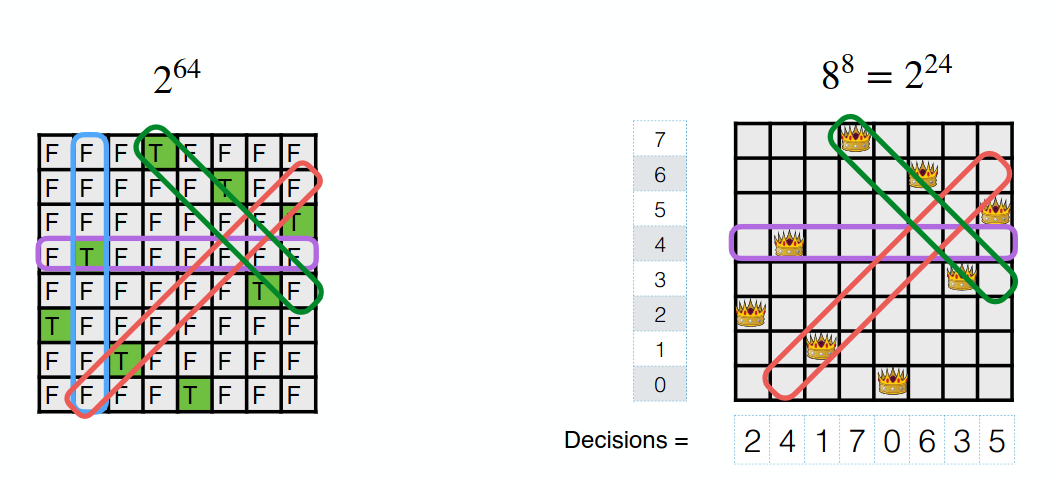
\includegraphics[width=0.8\textwidth]{img/Nqueens.png}
    \caption{N-queens problem: modeling comparison}
\end{figure}
The exploring of the variable assignment tree works as follows: at each node of the tree, we select a value to assign to the variable of the node from its domain. Then, we check whether the assignment satisfies all the constraints or not. If it does, we continue to explore the tree. Else, we backtrack (go back in the tree and change a previously assigned value to another) and try a different assignment for the variable. This process continues until we find a solution that satisfies all the constraints, or exhaust all the possible assignments. This is the most simple way to find a solution for a CP problem, but it corresponds to a brute force approach and not yet constraint programming. The spirit of CP is to do a search that leverages the structure of the solution space, instead of going through the whole graph like the brute force approach.
\section{How does CP work?}
To understand how CP works, let us consider a small example. We define three variables $x,y,z$ with domains $D_x = \{0,1\}$, $D_y = \{0,1,2\}$ and $D_z = \{0,1\}$; and the constraints $\texttt{AllDifferent(x,y,z)}$ and $x \geq z$. This corresponds for the moment to the brute force approach, and we will update this tree step by step to show how CP finds a solution faster. The exploration of the graph is done in a depth-first manner, we start from the root node and we explore the leftmost branch first, then when we reach a leaf, we backtrack and explore the next unexplored branch, and so on until we find a solution or exhaust the whole tree. The green leaf corresponds to a solution that satisfies all the constraints, while the orange leaf corresponds to a failure, meaning that the assignment of values to the variables does not satisfy all the constraints.
\begin{figure}[H]
\centering
    \begin{tikzpicture}[
        level distance=2.2cm,
        sibling distance=3.2cm,
        every node/.style={font=\small},
        var/.style={
            circle,
            draw,
            thick,
            minimum size=8mm,
            inner sep=1pt
        },
        fail/.style={
            circle,
            draw=orange,
            thick,
            minimum size=7mm,
            inner sep=1pt
        },
        success/.style={
            circle,
            draw=green!60!black,
            thick,
            minimum size=7mm,
            inner sep=1pt
        },
        edge from parent/.style={draw, thick},
        edge label/.style={font=\small, midway, fill=white, inner sep=1pt}
    ]
    % Tree
    \node[var] (x) at (0,0) {$x$};

    % x = 0 branch
    \node[var] (y0) at (-3.5,-1.5) {$y$};
    \draw[thick] (x) -- node[edge label, above left] {$x=0$} (y0);

    \node[fail] (f00) at (-6,-3) {};
    \draw[thick] (y0) -- node[edge label, above left] {$y=0$} (f00);

    \node[var] (z01) at (-3.5,-3) {$z$};
    \draw[thick] (y0) -- node[edge label, left] {$y=1$} (z01);

    \node[fail] (f010) at (-4.5,-4.5) {};
    \node[fail] (f011) at (-3.5,-4.5) {};
    \draw[thick] (z01) -- node[edge label, above left] {$z=0$} (f010);
    \draw[thick] (z01) -- node[edge label, above right] {$z=1$} (f011);

    \node[var] (z02) at (-1.5,-3) {$z$};
    \draw[thick] (y0) -- node[edge label, above right] {$y=2$} (z02);

    \node[fail] (f020) at (-1.5,-4.5) {};
    \node[fail] (f021) at (-0.5,-4.5) {};
    \draw[thick] (z02) -- node[edge label, above left] {$z=0$} (f020);
    \draw[thick] (z02) -- node[edge label, above right] {$z=1$} (f021);

    % x = 1 branch
    \node[var] (y1) at (3.5,-1.5) {$y$};
    \draw[thick] (x) -- node[edge label, above right] {$x=1$} (y1);

    \node[var] (z10) at (1.8,-3) {$z$};
    \draw[thick] (y1) -- node[edge label, above left] {$y=0$} (z10);

    \node[fail] (f100) at (1.1,-4.5) {};
    \node[fail] (f101) at (2.5,-4.5) {};
    \draw[thick] (z10) -- node[edge label, above left] {$z=0$} (f100);
    \draw[thick] (z10) -- node[edge label, above right] {$z=1$} (f101);

    \node[fail] (f11) at (3.5,-3) {};
    \draw[thick] (y1) -- node[edge label, right] {$y=1$} (f11);

    \node[var] (z12) at (5.5,-3) {$z$};
    \draw[thick] (y1) -- node[edge label, above right] {$y=2$} (z12);

    \node[success] (s120) at (4.8,-4.5) {};
    \node[fail] (f121) at (6.2,-4.5) {};
    \draw[thick] (z12) -- node[edge label, above left] {$z=0$} (s120);
    \draw[thick] (z12) -- node[edge label, above right] {$z=1$} (f121);

    \end{tikzpicture}
\end{figure}
Instead of going through the whole graph like above, CP is based on the propagation of the constraints. This means that, when assigning a value to a variable, we can use the constraints over the variables to reduce the other variable's domains. For example, if a constraint forces two variables to be different, and if a value is assigned to one of them, we can remove that value from the domain of the other variable. This helps find a solution faster by reducing the search space. The propagation of the constraints, is done based on the \texttt{Hollywood Principle} "Don't call us, we'll call you". This means that, instead of the search process calling the constraints to check whether an assignment is valid or not, the constraints will call the search process to notify it when a variable's domain has been reduced. This call can be done for 3 different events:
\begin{itemize}
    \item \textbf{Fixed value}: when a variable is assigned a value.
    \item \textbf{Domain reduction}: when a value is removed from a variable's domain.
    \item \textbf{Domain bounds reduction}: when the bounds of a variable's domain are reduced (less powerful than domain reduction but faster to compute).
\end{itemize} 
Going back to our example, we can easily observe that the left part of the tree will never be explored: when we fix $x=0$ and propagate the constraints, we immediately see that $D_z$ will be the empty set because the constraint $\texttt{AllDifferent}$ eliminate $z=0$ and the constraint $x \geq z$ eliminate $z=1$. This gives us the following tree.
\begin{figure}[H]
\centering
    \begin{tikzpicture}[
        level distance=2.2cm,
        sibling distance=3.2cm,
        every node/.style={font=\small},
        var/.style={
            circle,
            draw,
            thick,
            minimum size=8mm,
            inner sep=1pt
        },
        fail/.style={
            circle,
            draw=orange,
            thick,
            minimum size=7mm,
            inner sep=1pt
        },
        success/.style={
            circle,
            draw=green!60!black,
            thick,
            minimum size=7mm,
            inner sep=1pt
        },
        edge from parent/.style={draw, thick},
        edge label/.style={font=\small, midway, fill=white, inner sep=1pt}
    ]
    % Tree
    \node[var] (x) at (0,0) {$x$};

    \node[fail] (f00) at (-2.5,-1.5) {};
    \draw[thick] (x) -- node[edge label, above left] {$x=0$} (f00);

    % x = 1 branch
    \node[var] (y1) at (2.5,-1.5) {$y$};
    \draw[thick] (x) -- node[edge label, above right] {$x=1$} (y1);

    \node[fail] (f11) at (1.8,-3) {};
    \draw[thick] (y1) -- node[edge label, above left] {$y=0$} (f11);

    \node[var] (z12) at (3.2,-3) {$z$};
    \draw[thick] (y1) -- node[edge label, above right] {$y=2$} (z12);

    \node[success] (s120) at (3.9,-4.5) {};
    \draw[thick] (z12) -- node[edge label, above right] {$z=0$} (s120);

    \end{tikzpicture}
\end{figure}
In addition to the constraint propagation, it is possible to use branching heuristics: instead of exploring the tree in a depth-first manner, we can use heuristics to decide which variable to assign next and to which value. For example, the \textit{minimum remaining values heuristic} selects the variable with the smallest domain first, and the \textit{degree heuristic} selects the variable that is involved in the most constraints first. These heuristics can help find a solution faster by guiding the search process towards promising areas of the search space. Again, if we look at our example and apply the minimum remaining values heuristic (still with constraint propagation), we explore less nodes than with a simple lexicographic ordering. On the following graph, we first assign $x=1$ (because constraint propagation eliminates $x=0$). Then, we have $|D_y|=2$ and $|D_z| = 1$. Hence, we choose to assign $z$ first, and then $y$. We see that we explore less nodes using the heuristic than with the lexicographic ordering.
\begin{figure}[H]
\centering
    \begin{tikzpicture}[
        level distance=2.2cm,
        sibling distance=3.2cm,
        every node/.style={font=\small},
        var/.style={
            circle,
            draw,
            thick,
            minimum size=8mm,
            inner sep=1pt
        },
        fail/.style={
            circle,
            draw=orange,
            thick,
            minimum size=7mm,
            inner sep=1pt
        },
        success/.style={
            circle,
            draw=green!60!black,
            thick,
            minimum size=7mm,
            inner sep=1pt
        },
        edge from parent/.style={draw, thick},
        edge label/.style={font=\small, midway, fill=white, inner sep=1pt}
    ]
    % Tree
    \node[var] (x) at (0,0) {$x$};

    \node[fail] (f00) at (-2.5,-1.5) {};
    \draw[thick] (x) -- node[edge label, above left] {$x=0$} (f00);

    % x = 1 branch
    \node[var] (y1) at (2.5,-1.5) {$z$};
    \draw[thick] (x) -- node[edge label, above right] {$x=1$} (y1);

    \node[var] (z12) at (3.2,-3) {$y$};
    \draw[thick] (y1) -- node[edge label, above right] {$z=0$} (z12);

    \node[success] (s120) at (3.9,-4.5) {};
    \draw[thick] (z12) -- node[edge label, above right] {$y=2$} (s120);

    \end{tikzpicture}
\end{figure}
\subsection{Fixpoint algorithm}
To find a CP solution, we will repeatedly apply the following steps when we assign a value to a variable:
\begin{itemize}
    \item select a constraint (can be chosen smartly based on heuristics)
    \item check if it is infeasible with the current variable assignment, if it is, we backtrack and try a different assignment for the variable.
    \item if it is feasible, we propagate the constraint to reduce the domains of the other variables.
    \item repeat the process until no constraint can remove any value
\end{itemize}
This is a fixpoint algorithm. 
\subsection{State management and backtracking}
As said before, when we assign a value to a variable and we observe an inconsistency (infeasibility), we need to backtrack and try a different assignment for the variable. To do this, we need to keep track of the state of the search process, which includes the current variable assignments and the current domains of the variables. When we backtrack, we need to restore the previous state of the search process before trying a different assignment for the variable. A naive way to do this is to copy the entire state of the search process before making an assignment, and then restore it when we backtrack. However, this can be very inefficient in terms of memory and time. Instead, we can use a more efficient way to manage the state of the search process by using only copying the domain that changes for example. For example, TinyCSP works as follows:
\begin{itemize}
    \item clone the current domains,
    \item branch, for example $y = v$,
    \item apply fixpoint propagation,
    \item if the branch fails or ends, restore the cloned domains,
    \item try the other branch, for example $y \neq v$.
\end{itemize}
\subsection{Heuristics}
In CP, heuristics play a crucial role in guiding the search process towards promising areas of the search space. CP is based on the first fail principle, which means that if a branch is going to fail, we want to detect it as early as possible. There are several types of heuristics that can be used in CP, the most basics are as cited before:
\begin{itemize}
    \item \textbf{Minimum Remaining Values}: selects the variable with the smallest domain first. The idea is that if a variable has a small domain, it is more likely to lead to a failure, and thus we want to assign it first to detect failures early.
    \item \textbf{Degree Heuristic}: selects the variable that is involved in the most constraints first. The idea is that if a variable is involved in many constraints, it will propagate more constraints, and thus possibly find a failure fast, so we want to assign it first to detect failures early.
\end{itemize}
\chapter{MiniCP architecture}
MiniCP is a constraint programming solver that is designed to be simple and easy to understand, it is the solver used in this course. So in order to understand well CP and how to use it, it is important to understand how MiniCP works.
\begin{definition}
    A \textbf{domain} is a finite set of integers that represents the still possibles values for a variable.
\end{definition}
We can query this set (\texttt{min()}, \texttt{max()}, \texttt{size()}, ...), remove values from it but we cannot add values to it. We can also detect if it is empty or if the value of the variable is fixed (i.e. the domain contains only one value). MiniCP uses \textbf{sparse set} to represent the domains, especially because the removal of a value is done in constant time with this data structure. The sparse set uses two arrays and one integer:
\begin{itemize}
    \item \texttt{values}: an array that contains the values of the domain, the values are not necessarily in order.
    \item \texttt{index}: an array that contains the index of each value in the \texttt{values} array.
    \item \texttt{size}: an integer that represents the size of the domain.
\end{itemize}
Example with:
\begin{lstlisting}
    values = [0, 1, 2, 3, 8, 5, 6, 7, 4]
    index = [0, 1, 2, 3, 8, 5, 6, 7, 4]
    size = 8
\end{lstlisting}
Then the value 4 is not in the domain because it is not in the first 8 values of the \texttt{values} array. To remove a value from the domain, we swap it with the last value in the \texttt{values} array and decrease the size by 1. For example, if we want to remove the value 2, we swap it with the last value inside the domain, which is 7, and we decrease the size by 1, which gives us:
\begin{lstlisting}
    values = [0, 1, 7, 3, 8, 5, 6, 2, 4]
    index = [0, 1, 7, 3, 8, 5, 6, 2, 4]
    size = 7
\end{lstlisting}
This way, we can remove a value from the domain in constant time. To check if a value is in the domain, we can check if its index in the \texttt{index} array is less than the size of the domain. For example, to check if the value 3 is in the domain, we check if \texttt{index[3]} is less than \texttt{size}, which is true because \texttt{index[3]} is 3 and \texttt{size} is 7. To check if the value 4 is in the domain, we check if \texttt{index[4]} is less than \texttt{size}, which is false because \texttt{index[4]} is 8 and \texttt{size} is 7.
\section{Stateful objects}
During the search process, the solver will take decision that will modify the domains but if the branch fails, we need to backtrack and restore the previous state of the domains. To do this, MiniCP uses stateful objects, which are objects that can save and restore their state. Each stateful object is kept in the \textbf{State Manager} of MiniCP, which is responsible for saving and restoring the state of the objects when we backtrack. Domains are not the only stateful objects in MiniCP, we also have stateful integers such as the size of the domain, the number of variables that are not yet assigned, etc. There is two ways to manage state, the copier method and the trailer method. The copier method consists in copying all the stateful objects when \texttt{saveState()} is called and restores the full snapshot when \texttt{restoreState()} is called. The copier methods has the advantage of being simple to implement and highly parallelisable but it is expensive if there is many stateful objects and not very efficient as it copies the whole state even if only one value change. On the other hand, the trailer method initialize a new empty backup with \texttt{saveState()} and when a stateful object changes, it saves the previous value of the object in the backup. When \texttt{restoreState()} is called, it restores all the values in the backup. The trailer method is more efficient than the copier method because it only saves the values that change, but it is more complex to implement and harder to parallelise. 
\section{IntDomain ADT}
MiniCP uses a generic interface for the domains, called \texttt{IntDomain}, which defines the operations that can be performed on the domains. This Abstract Data Type allows us to have different implementations of the domains, such as a sparse set, an interval, etc. The \texttt{IntDomain} interface defines the following operations:
\begin{itemize}
    \item \texttt{min()}: returns the minimum value of the domain.
    \item \texttt{max()}: returns the maximum value of the domain.
    \item \texttt{size()}: returns the size of the domain.
    \item \texttt{contains(int v)}: returns true if the value v is in the domain, false otherwise.
    \item \texttt{isSingleton()}: returns true if the domain contains only one value, false otherwise.
    \item \texttt{remove(int v, DomainListener l)}: removes the value v from the domain.
    \item \texttt{removeAllBut(int v, DomainListener l)}: removes all values from the domain except v.
    \item \texttt{removeBelow(int v, DomainListener l)}: removes all values from the domain that are less than v.
    \item \texttt{removeAbove(int v, DomainListener l)}: removes all values from the domain that are greater than v.
\end{itemize}
\section{DomainListener}
A \texttt{DomainListener} is an object that listens to the changes in the domain of a variable. When a value is removed from the domain of a variable, the \texttt{DomainListener} is notified and can react to this change. The domain listeners will react to differents events such as: empty domain, fixed value, domain reduction, domain bounds reduction. For example, if we have a constraint that says that two variables must be different, and if we assign a value to one of the variables, the domain listener of the other variable will be notified and will remove that value from its domain. This way, we can propagate the constraints and reduce the search space.
\section{Variables}
In MiniCP, a variable is represented by the \texttt{IntVar} class, which contains a reference to the solver, a domain, and track the constraints that involve this variable. Then there is an API for the variables that allows us to perform queries on them, such as getting their size, if it contains a variable, if it is fixed, etc. We can also perform updates on the variables, such as removing a value from their domain, fixing their value, etc. And finally, there is hookups, which register the constraints that needs to be notified when the variable's domain changes. For example, if we have a constraint that says that two variables must be different, we will register this constraint as a hookup for both variables, so that when we assign a value to one of the variables, the constraint will be notified and will remove that value from the domain of the other variable. We have 3 types of hookups:
\begin{itemize}
    \item \texttt{propagateOnDomainChange(c)}
    \item \texttt{propagateOnBoundsChange(c)}
    \item \texttt{propagateOnFix(c)}
\end{itemize}
The boolean variables are implemented as a special case of the integer variables, they have a domain that contains only two values: 0 and 1. They are called \texttt{BoolVar} and have some specific methods such as \texttt{isTrue()} and \texttt{isFalse()}.  
\subsection{Variable views}
To avoid duplicating code for constraints that are similar but not identical, MiniCP uses variable views. A variable view is a variable that is derived from another variable, called the base variable. A view is a fake variable that behaves like a normal variable but depends on another variable. For example, we can have a view that represents the negation of a variable, or a view that represents a variable but shifted. 
\begin{lstlisting}
    D(X) = {0, 1, 2, 3}
    Y = X + 2
\end{lstlisting}
Then if we ask \texttt{Y.contains(5)} it translates to \texttt{X.contains(3)}.
These views are thus useful to avoid duplicating code for constraints. For example instead of having a code for the constraint $X \neq Z$ and another code for the constraint $X + 2 \neq Z$, we can have a view $Y = X + 2$ and then use the same code for the constraint $Y \neq Z$. 
\section{Constraint scheduling}
A variable stores constraints in three stacks: onDomain, onFix and onBounds. So when the domain listener detects an event, it schedules the corresponding constraints in the corresponding stack. These stacks are stateful stacks that are composed of an Arraylist containing the constraints and an integer that represents the size of the stack. When we schedule a constraint, we add it to the stack and increase the size by 1. When we propagate a constraint, we remove it from the stack and decrease the size by 1. And when we backtrack, we restore the size of the stack to the previous value, which means that we restore the previous state of the stack. This way, we can manage the scheduling of the constraints efficiently and correctly during the search process.
\section{Constraints}
A constraint implements a filtering algorithm, it has two main methods: \texttt{propagate()} and \texttt{post()}. The \texttt{post()} method is called when the constraint is added to the solver, it is responsible for initializing the constraint and to register them on the variables it depends on and for doing some initial propagation. The registration is called a hookup. On the other part, the \texttt{propagate()} method is called when the constraint is scheduled, it is responsible for filtering the domains of the variables it depends on. For example, if we have a constraint that says that two variables must be different, the \texttt{propagate()} method will remove the value of one variable from the domain of the other variable when one of them is assigned a value. The \texttt{propagate()} method can also detect if the constraint is infeasible or if it is already satisfied, in which case it can return a failure or a success respectively. The constraints also have two attributes: \texttt{active} and \texttt{scheduled}. The \texttt{active} attribute indicates whether the constraint is active or not, if it is not active, it means that the constraint is already satisfied and thus it does not need to be propagated anymore. The \texttt{scheduled} attribute indicates whether the constraint is already scheduled or not, if it is already scheduled, it means that it is already in the propagation queue and thus it does not need to be scheduled again.
\section{Solver and propagation queue} 
The solver is the main class of MiniCP, it orchestrates everything. The solver interface contains methods to construct the model (post constraints, objective) and then an API for the search process (schedule constraints, fixpoint methods). The \texttt{schedule(c)} method is used to schedule a constraint, it adds the constraint to the propagation queue but only if the constraint is active and if the constraint is not already in the queue to avoid duplicate propagation. The \texttt{propagate()} method removes a constraint in the queue and propagates it. And finally, the \texttt{fixpoint()} method repeatedly calls the \texttt{propagate()} method until the queue is empty, which means that no constraint can further reduce the domains of the variables. If a contradiction occurs, the queue is cleared and an exception is thrown to signal the failure of the current branch. The fixpoint is reached when no scheduled constraint can remove more values.
\section{Search tree}
The search tree is explored through branching decisions, which are made by the search process. A branching decision split the search space into two or more subspaces, for example, we can have a branching decision that creates two branches: one where a variable is assigned a value ($X = 1$), and another where that variable is not assigned that value ($X \neq 1$). This is valid because no solution is lost and no solution is explored twice. We can have different types of branching decisions, such as $X \leq 1$ and $X > 1$, or one branch for each value in the domain of a variable.\\
This search tree is explored in a depth-first manner, we start from the root node and we explore the leftmost branch first, then when we reach a leaf, we backtrack and explore the next unexplored branch, and so on until we find a solution or exhaust the whole tree. The search process can also use heuristics to decide which variable to assign next and to which value, as explained before. The DFS has been chosen because it is simple, uses little memory and naturally fits with the backtracking process.\\
The searching process has 3 states:
\begin{itemize}
    \item \textbf{Success}: if all variables are fixed then a solution is found, and the search process can stop.
    \item \textbf{Failure}: if a variable has an empty domain, then the current branch is infeasible, and the search process needs to backtrack and try a different assignment for the variable.
    \item \textbf{Not finished}: if there are still variables that are not fixed and there are still values in their domains, then the search process needs to continue exploring the tree.
\end{itemize}
We can also asks the search process to find all solutions, in this case, when a solution is found, the search process will not stop but will backtrack and continue exploring the tree to find other solutions.
\chapter{Constraints design}
\section{Consistency of a constraint}
\subsection{Domain consistency (DC)}
\begin{definition}
    A constraint is \textbf{domain consistent} if every value in the domain of every variable participates in at least one solution of the constraint.
\end{definition}
So for example if we have a constraint $X = Y + 1$ and $D_X = \{1,2,3\}$ and $D_Y = \{0,1\}$, then the constraint is not domain consistent because the value 3 in $D_X$ does not participate in any solution of the constraint. To make it domain consistent, we need to remove the value 3 from $D_X$, which gives us $D_X = \{1,2\}$ and $D_Y = \{0,1\}$. Domain consistency is a strong form of consistency, it can be expensive to achieve but it can also lead to a significant reduction of the search space. The complexity to achieve domain consistency is the sum of the size of the domains of the variables involved in the constraint ($\mathcal{O} (\sum_{i} |D_i|)$). 
\subsection{Bound consistency (BC)}
\begin{definition}
    A constraint is \textbf{bound consistent} if for every variable, the minimum and maximum values of its domain participate in at least one solution of the constraint.
\end{definition}
Bound consistency is a weaker form of consistency than domain consistency, it is less expensive to achieve but it can also lead to a less significant reduction of the search space. 
\section{Sum constraint}
The sum constraint is a very common constraint in CP, it is used to express that the sum of a set of variables must be equal to a given value. For example, if we have a set of variables $X_1, X_2, X_3$ and we want to express that their sum must be equal to $y$ (an arbitrary value), we can write the constraint as follows:
\begin{lstlisting}    
    sum(X) = y
\end{lstlisting}
Achieving domain consistency for the sum constraint is a NP-hard problem, so usually we will use bound consistency for this constraint. To achieve bound consistency for the sum constraint, we want that the equality holds for the minimum and maximum values of the domains of the variables. So we want that $y$ is between the minimum and maximum values of the sum of the variables, which gives us the following inequalities:
\begin{equation}
    \sum_{i} \min(D_i) \leq y \leq \sum_{i} \max(D_i)
\end{equation}
From these inequalities, we can derive a naive filtering formula for each variable $X_i$:
\begin{equation}
    \begin{aligned}
        \min(D_i) = \max(\min(D_i), y - \sum_{j \neq i} \max(D_j))\\
        \max(D_i) = \min(\max(D_i), y - \sum_{j \neq i} \min(D_j))
    \end{aligned}
\end{equation}
So for the following example:
\begin{lstlisting}
    X1 in [-100, 10]
    X2 in [4, 6]
    X3 in [20, 60]
    sum(X) = 0
\end{lstlisting}
We have $X2 + X3 \in [24, 66]$, so we can deduce that $X1 \in [-66, -24]$ to satisfy the sum constraint. So this filtering algorithm is in $\Theta(n)$ for each variable. Doing this at each propagation step can be expensive, so we can precompute thoses values and just update them when the domains of the variables change.
\subsection{Incremental Sum Propagator}
The idea of the incremental sum propagator is to keep track of the sum of the fixed values of the variables. The propagator keep two state integer and a stateful sparse set:
\begin{itemize}
    \item \texttt{sumFixed}: the sum of the fixed values of the variables
    \item \texttt{nFixed}: the number of fixed variables
    \item \texttt{unFixed}: a sparse set that contains the indices of the unfixed variables
\end{itemize}
So each time it is propagated, it updates the sum of the fixed values and the number of fixed variables, and it updates the sparse set of the unfixed variables. And thus we can easily compute the minimum and maximum values of the sum of the unfixed variables, which allows us to apply the filtering formula for each variable easily.
\begin{definition}
    A propagator is \textbf{idempotent} if applying it twice does not change the result after the first application. 
\end{definition}
If a propagator is idempotent, it means that we only need to apply it once to reach a fixpoint, which can save a lot of time during the search process. The incremental sum propagator is idempotent because it only updates the sum of the fixed values and the number of fixed variables, and it does not change the domains of the variables directly. So applying it twice will not change the result after the first application.\\
But if we allow variables views, almost no filtering algorithm remains idempotent because the views can change the domains of the variables in a way that can trigger the propagator to be applied again. 
\section{Element constraint}
The element constraint allows us to index an array using a variable, so the indexes and the values of the array are variables. The basic 1D element constraint can be written as follows $T[y] = z$:
\begin{lstlisting}
    T = [3, 4, 5, 5, 4, 3]
    D(y) = {0,1,2,3,4,5}
    D(z) = {3,4,5}
\end{lstlisting}
Where $T$ is an array of variables, $y$ is a variable that represents the index of the array, and $z$ is a variable that represents the value of the array at the index $y$. With this, a propagator could filter in both directions. From $z$ to $y$ if $T[i] \notin D(z)$ then remove $i$ from $D(y)$, and from $y$ to $z$ if $\forall i \in D(y)$ there is no value $v$ then remove $v$ from $D(z)$.\\
But the most interresting part of the element constraint is the 2D version, which can be written as follows $T[x][y] = z$. This 2D formulation is useful for problems such as the Quadratic Assignment Problem (QAP) because in the formulation of the QAP the objective function will look like this: $\sum_{i,j} f_{ij} D[i][j]$ where $f_{ij}$ is the flow between facilities $i$ and $j$, $D[i][j]$ is a 2D element constraint. 
\subsection{Propagation}
To propagate the 2D element constraint efficiently, we want first to represent all possible combinations of $T[x][y] = z$ by some tuples $(z,x,y)$ that are sorted by $z$ then $x$ then $y$. The propagator keep tracks of the first and last valid tuples, it also keeps track of the support of $x$ and $y$. When a tuple is invalidated, we update the support of $x$ and $y$, and if the support of $x$ or $y$ is empty, we remove the corresponding value from their domain. This propagation works also in 1D format. 
\subsection{Element over an array of variable}
So far, $T$ was an array of constants, but we can also have $T$ as an array of variables, which means that we have $T[y] = z$ where each $T[i]$ is a variable. This appears in models such as stable matching.\\
For this kind of constraint, the most efficient approach for consistency is to use an hybrid domain consistency, where we enforce domain consistency on the index variable $y$ and bound consistency on the value variable $z$ and $T[i]$. So for the filtering algorithm, we first want to filter $y$ then we want to filter $z$ and finally $T[i]$ but only if $y$ is fixed. To filter $y$, we want that for each $i \in D(y)$, if $D(T[i]) \cap D(z) = \emptyset$ then we remove $i$ from $D(y)$. To filter $z$, we want to update the bounds using all possible $T[i]$ where $i \in D(y)$:
\begin{equation}
    \begin{aligned}
        \min(z) \geq min_{i \in D(y)} \min(D(T[i]))\\
        \max(z) \leq max_{i \in D(y)} \max(D(T[i]))
    \end{aligned}
\end{equation}
And then the filtering of $T[i]$ is only done if $y$ is fixed. Then we can propagate the equality $T[i]=z$.\\
But if we want to achieve domain consistency, we can filter $z$ by checking for each value $v \in D(z)$ if there is no $i \in D(y)$ such that $v \in D(T[i])$, then we can remove $v$ from $D(z)$. This is more expensive than the bound consistency filtering because intersection between sparse sets can be expensive, but it can lead to a significant reduction of the search space. 
\section{Table constraint}
A table constraint is a constraint that represents a relation between a set of variables by explicitly listing the allowed combinations of values for those variables. The idea is that only one combination of values is allowed for the variables. For example, if we have three variables $X, Y, Z$ and each variable has a domain of $\{0,1\}$, we can have a table constraint that allows only the following combinations of values:
\begin{center}
    \begin{lstlisting}    
        (X=0, Y=0, Z=0)
        (X=0, Y=0, Z=1)
        (X=0, Y=1, Z=0)
        (X=0, Y=1, Z=1)
        (X=1, Y=0, Z=0)
        (X=1, Y=0, Z=1)
        (X=1, Y=1, Z=0)
        (X=1, Y=1, Z=1)
    \end{lstlisting}
\end{center}
which gives us the following table:
\begin{center}
    \begin{tabular}{c|c|c}
    X & Y & Z \\
    \hline
    0 & 0 & 0 \\
    0 & 0 & 1 \\
    0 & 1 & 0 \\
    0 & 1 & 1 \\
    1 & 0 & 0 \\
    1 & 0 & 1 \\
    1 & 1 & 0 \\
    1 & 1 & 1 \\
    \end{tabular}
\end{center}
We can represent this table constraint as a logic formula as follows:
\begin{equation}
    (X=0 \land Y=0 \land Z=0) \lor (X=0 \land Y=0 \land Z=1) \lor \dots \lor (X=1 \land Y=1 \land Z=1)
\end{equation}
This formulation where we explicitly list all the allowed combinations of values is called an \textbf{extensional formulation}. On the contrary, if we have a formulation where we express the relation between the variables by using some mathematical expressions or logical formulas, it is called an \textbf{intensional formulation}. In general, if we have an efficient intensional constraint with domain consistency then we should prefer this instead of the extensional formulation. The extensional formulation can be useful when we have a relation that is hard to express with an intensional formulation but for some formulation this can be very inefficient. For example for an all different constraint, for $n$ variables with a domain of size $n$, we have $n!$ allowed combinations of values, which can be very large even for small values of $n$.\\
Element 2D constraint can be written as a table constraint because asking for $T[x][y] = z$ is equivalent to asking for $(x,y,z) \in$ table. 
\subsection{Filtering}
A valid tuple in the table is a tuple that is still possible given the current domains of the variables, which means that all the elements of the tuple are in their respective domains. To filter the table constraint, we want to remove the values from the domains of the variables that do not participate in any valid tuple. So for a value $v$ in the domain of a variable $X_i$, if there is no valid tuple that contains $v$ in the table, we remove $v$ from $D(X_i)$.\\
A slow way to filter the table constraint can be done with this little algorithm:
\begin{lstlisting}    
    for each variable X_i:
        for each value v in D(X_i):
            if there is no valid tuple that contains v in the table:
                remove v from D(X_i)
\end{lstlisting}
A faster way is to use \texttt{STR2} algorithm (Simple Tabular Reduction). This algorithm scans the valid tuples and collects supports. The algorithm is as follows:
\begin{lstlisting}
    SupportedValues = empty set
    for each tuples in table:
        if the tuple is valid:
            for each variable X_i in the tuple:
                add the value of X_i in the tuple to SupportedValues
        else: 
            remove the tuple from the table
    for each variable X_i:
        for each value v in D(X_i):
            if v not in SupportedValues:
                remove v from D(X_i)
\end{lstlisting}
The important idea is that STR2 gets incrementality from the table itself. The invalid tuples removed will thus not be scanned again in the next propagation. The STR2 algorithm needs a stateful table to keep track of the valid tuples and be able to restore the invalided ones. The stateful table works like a sparse set, we have a state int that represents the size of the table and an array that contains the tuples. When we remove a tuple, we swap it with the last valid tuple in the array and decrease the size by 1. When we backtrack, we restore the size of the table to the previous value.\\
\textcolor{red}{Add compact table filtering algorithm}
\section{AllDifferent constraint}
Formally, the all different constraint is defined as follows:
\begin{equation}
    \forall i,j \in \{1, \dots, n\}, i \neq j \Rightarrow X_i \neq X_j
\end{equation}
\subsection{Binary decomposition}
The easiest way to implement the all different constraint is to decompose it into binary constraints, which means that we will have a binary constraint $X_i \neq X_j$ for each pair of variables $X_i$ and $X_j$. This decomposition is easy to implement but it is not very efficient because it uses $n(n-1)/2$ binary constraints for $n$ variables.\\
\subsection{Forward checking (FWC)}
The \textbf{Forward checking (FWC)} is the filtering algorithm obtained from the binary decomposition, it is a simple algorithm that only removes the fixed value from the domains of the other variables when a value is fixed to a variable. This algorithm is not very strong because it does not detect any inconsistency until a variable is fixed, which means that it can explore a lot of the search space before finding a failure. For example, if we have 3 variables $X_1, X_2, X_3$ with domains $\{1,2\}$ and we have the all different constraint on them, then the forward checking algorithm will not detect any inconsistency until we assign a value to 2 of the variables. 
\subsection{Global AllDifferent}
Instead of posting many not equal constraints, we can post a global all different constraint. The idea is to separate the variables into two parts the fixed variables and the unfixed variables throught a stateful sparse set of indices and a stateful int (nFixed). The idea is that when a variable is fixed, we move it in the fixed part of the sparse set and we remove its value from the domains of the unfixed variables and update the nFixed value. This algorithm uses a form of forward checking algorithm, this gives us a filtering algorithm that is not stronger than the binary decomposition but faster.
\subsection{Feasibility check}
We saw in the FWC algorithm that we can hardly detect an inconsistency due to the fact that we have too little values for the number of variables. To detect this inconsistency, we can build a bipartite graph between the value and variable. Using this graph, we know that AllDifferent is feasible if and only if there exists a matching of size $n$ that covers all variables. It means that we want to find a maximum matching of size $n$ and that if it does not exist, then we can conclude that the constraint is infeasible.\\
An efficient algorithm to find a maximum matching in a bipartite graph is the \textbf{Alternating Path} algorithm, this algorithm is based on the idea of finding an augmenting path in the graph, which is a path that alternates between edges that are in the matching and edges that are not in the matching. If the path starts from an unmatched variable and ends at an unmatched value, then flipping the edges increases the size of the matching. A matching M is maximum if and only if no augmenting alternating path exists.
\subsection{Domain consistency}
Domain consistency for the all different constraint implies that a value $v$ can stay in $D(X)$ if and only if there exists at least one complete assignment where $X = v$ and all other variables are assigned different values. So using the graph representation, we want to remove every edge that does not belong to any maximum matching of size $n$. So we want to remove value $v$ from $D(X)$ if edge $(X,v)$ does not belong to any maximum matching of size $n$.\\
The naive idea would be enumerating all the maximum matching of size $n$ and removing the edges that do not belong to any of them, but this is not efficient because there can be exponentially many maximum matchings. The efficient way to do this is to use the following theorem: 
\begin{thm}[Berge’s theorem]
    For an arbitrary maximum matching M, an edge belongs to some maximum matching if it is:
    \begin{itemize}
        \item already in M, or
        \item  part of an even-length alternating path starting from an M-free node, or
        \item part of an even-length alternating cycle.
    \end{itemize}
    An M-free node is a node that is not matched by the matching M.
\end{thm}
\textcolor{red}{maybe add algo}\\
Another idea to have an efficient filtering algorithm is to use the strongly connected components. Strongly connected component is a maximal set of nodes where every node can reach every other node throught directed paths. In a directed graph, an edge is part of a directed cycle if its endpoints belong to the same SCC. There is an algorithm created by Régin to take profit of the SCC:
\begin{enumerate}
    \item Compute a maximum matching M
    \item Build the directed graph
    \item Compute the SCC
    \item Remove edges that are not in M and whose endpoints are in differents SCC
\end{enumerate}
This gives domain consistency for the all different constraint. The full Régin's filtering algorithm works like this:
\begin{enumerate}
    \item Build the variable-value graph.
    \item Compute a maximum matching M that covers all variables.
    \item If no such matching exists, fail.
    \item Build the residual directed graph from M.
    \item Add the dummy node to merge path and cycle cases.
    \item Compute SCCs.
    \item For every edge (x, a):
    \begin{itemize}
        \item if (x, a) is not in M and x and a are in different SCCs:
        \begin{itemize}
            \item remove a from D(x)
        \end{itemize}
    \end{itemize}
\end{enumerate}
The advantages of matching is that a matching found is still valid after a backtracking step.
\subsection{Global Cardinality Constraints (GCC)}
The global cardinality constraint is a generalization of the all different constraint, where it is allowed to have multiple variables assigned to the same value, but we want to limit the number of variables that can be assigned to each value. 
\section{Circuit constraints}
The Circuit constraint enforces a Hamiltonian cycle on an array of successor variables. This consists in an array $succ$ reprensenting the successor of each node in the cycle, and we want to enforce that there is a cycle that goes through all the nodes. Let us consider the following example:
\begin{figure}[H]
    \centering
    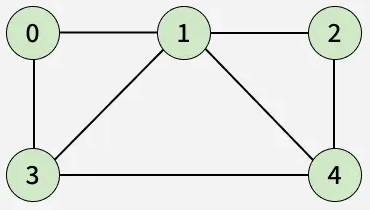
\includegraphics[width=0.5\textwidth]{img/ham.png}
\end{figure}
For this graph, we have an Hamiltonian cycle that goes through all the nodes counterclockwise starting from node 0, with this we would have the following successor variables:
\begin{lstlisting}
    succ = [3, 0, 1, 4, 2]
\end{lstlisting}
This successors array means that every node is visited exactly once and we get one complete cycle. This circuit constraint is useful for problems such as the Traveling Salesman Problem (TSP) and the Vehicle Routing Problem (VRP).
\subsection{Filtering}
The Hamilton cycle problem is NP-complete, so achieving domain consistency for the circuit constraint is NP-hard.\\
A first approach is \textbf{degree reasoning}, this approach is based on the idea that in an Hamiltonian cycle, each node must have exactly one successor and one predecessor. This gives two filtering rules:
\begin{itemize}
    \item \textbf{Fixed successor:} If $D(succ[i]) = \{j\}$, then node $i$ is forced to go to node $j$, so we can remove $j$ from the domains of the successors of all other nodes. This is similar to the forward checking algorithm for the all different constraint.
    \item \textbf{Unique predecessor:} If $D^{-1}(j) = \{i\}$, then node $j$ is forced to have node $i$ as its predecessor, so we must enforce $succ[i] = j$.
\end{itemize}
This filtering is fast but not very strong, it can be useful to quickly reduce the search space but it will not detect many inconsistencies. For example, it won't detect sub-cycles.\\
Another approach is to use \textbf{partial-path-based filtering}. A partial path is a maximal sequence of nodes connected by fixed successors variables. If this path is not yet covering all the nodes, then we must not close it into a cycle. So if the path is smaller than $n-1$ then $succ[dest] \neq orig$.\\
For this partial-path-based filtering, we want to store 3 values for each node $i$: 
\begin{itemize}
    \item $dest[i]$: destination of the partial path starting from node $i$.
    \item $succ[i]$: successor of node $i$ (if not fixed then $succ[i] = i$).
    \item $lengthToDest[i]$: number of edge from $i$ to $dest[i]$.
\end{itemize} 
These values allow the propagator to merge the partial paths efficiently by updating the values when a new successor is fixed.\\
This partial-path-based filtering is not idempotent because the merging of the partial paths can trigger new filtering. To make this filtering incremental and proper to propagation, we need to keep track of the changes in the partial paths variable and thus make them stateful.\\
\subsection{Feasibility check}
To check the feasibility of the circuit constraint, we can use the fact that the circuit constraint is feasible if and only if every node is in the same strongly connected component. This is because a circuit exists if and only if there is a path from every node to every other node, which means that all nodes are in the same strongly connected component.
\chapter{Optimization}
For a CP optimization problem, the algorithm is implemented in a way such that it always converges to a global optimum. Indeed, a CP optimization problem is solved by finding a feasible solution, and then adding a constraint on the objective value to exclude that solution, enforcing the algorithm to find a better solution. Moreover, CP is well suited for problems where the relations between the variables are difficult to express with purely linear relationships. For example, the \texttt{AllDifferent} constraint ensures all variables have different values, which is hard to efficiently express linearly because it requires lots of slack variables. In comparison with Mixed Integer Linear Programming, CP is often more natural when the model contains many logical relations, conditional decisions, or complex discrete patterns that would require many auxiliary variables and big-M formulations in a linear model. Both CP and MILP have their strengths, the latter being stronger with linear relaxation. However, CP is often stronger when the main difficulty lies in discrete feasibility and logical structure.\\
CP can be very strong for proving optimality because of it's way of searching for better solutions, but it can have weaknesses such as:
\begin{itemize}
    \item the search tree can be huge,
    \item optimization problems can be very hard,
    \item the solver may spend too much time exploring unpromising regions,
    \item good solutions may be found deep in the search tree.
\end{itemize}
\section{Branch and bound}
CP works like a branch and bound algorithm for optimization problems. The search process follows this idea:
\begin{enumerate}
    \item Find a feasible solution using the search process.
    \item If a solution is found, add a constraint to the model that excludes this solution by enforcing the objective value to be better than the value of the found solution.
    \item Repeat the search process to find a better solution until no better solution is found.
\end{enumerate}
With this algorithm, we are guaranteed to find the global optimum because we are always excluding the current solution and looking for a better one.\\ 
Throughout the search process, we need to keep track of the current objective value so we will define it as a stateful variable. This value will kept on track by two listenners:
\begin{itemize}
    \item \texttt{onSolution}: this listener is called when a solution is found, it thightens the objective value to be better than the current solution.
    \item \texttt{onFixPoint}: at each fixpoint, the objective variable is restricted using the current bound.
\end{itemize}
\subsection{Large Neighborhood Search (LNS)}
The weaknesses of optimization with CP cited before motivates the need of heuristics to guide the search process towards promising regions of the search space. One of these heuristics is the Large Neighborhood Search (LNS), which is a metaheuristic mixing CP and local search.\\
The idea of LNS is to avoid being stuck in a local optimum and wasting time improving little by exploring other solutions that are far away from the current solution. Let us consider the exploring of a search space as a tree, here represented by a triangle:
\begin{figure}[H]
    \centering
    \begin{subfigure}{.5\textwidth}
        \centering
        
\includegraphics[width=\linewidth]{img/lns1.png}
        \caption{Without LNS}
    \end{subfigure}%
    \begin{subfigure}{.5\textwidth}
        \centering
        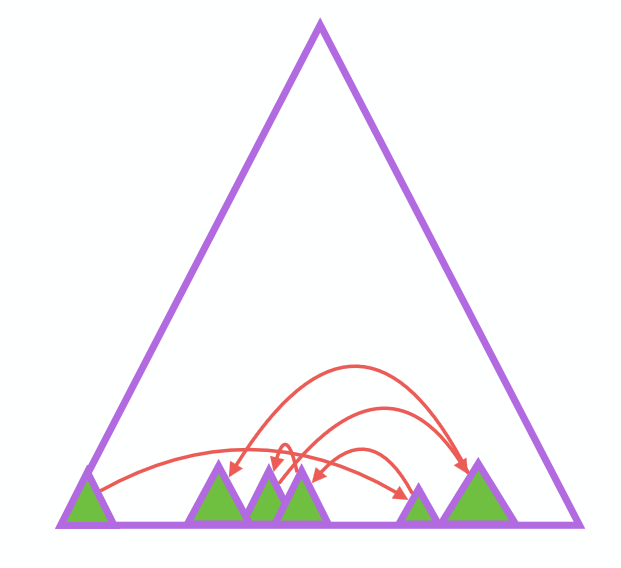
\includegraphics[width=\linewidth]{img/lns2.png}
        \caption{With LNS}
    \end{subfigure}
    \caption{Comparison of search space exploration with and without LNS}
\end{figure}
On the left side, we can see that without LNS, the search process could be stuck on the left branch of the tree and could explore the whole tree before finding the solution. Where on the right side, we can see that with LNS, the search process can explore multiple other highly different solutions which can lead faster to a better solution.\\
The principle of LNS contains 3 main steps:
\begin{enumerate}
    \item \textbf{Fix}: we randomly fix a subset of the variables to their values in the current solution. This is done by adding constraints to the model that enforce the fixed variables to take their values in the current solution.
    \item \textbf{Relax}: we relax the other variables and let them free to take any value in their domain.
    \item \textbf{Restart}: we restart the search process to find a better solution with the new constraints.
\end{enumerate}
The proportion of variables to fix is a parameter that we can tune to balance between exploration and exploitation. If we fix too many variables, we may not explore enough of the search space, but if we fix too few variables, we may not exploit enough of the current solution.\\
The specific part that makes LNS interesting is the fact that we relax a whole set of variables at once, which allows us to escape local optima.\\
In addition we can add a \textbf{limit of failure} to avoid spending too much time on unpromising regions of the search space. Like the proportion of fixed values, this limit of failure is a parameter that we can tune to balance between exploration and exploitation. The limit of failure represents the maximum number of inconsistent branches found during a restart before giving up and trying a different subset of variables to fix. If the limit of failure is too low, we may give up too quickly on promising regions of the search space, but if it is too high, we may spend too much time on unpromising regions.
\chapter{Scheduling}
Scheduling means allocating scarce resources to activities over time. In Constraint Programming, scheduling problems are important because CP offers:
\begin{itemize}
    \item high-level modeling abstractions, such as activities, start times, durations, resources;
    \item strong filtering algorithms to reduce the search tree;
    \item good search strategies to decide which activity to schedule first.
\end{itemize}
Scheduling is commonly structured as a problem where activities must be placed in time while respecting limited resources.
\section{Activity attributes}
A scheduling activity $i$ is defined by the following attributes:
\begin{itemize}
    \item $s[i]$: the start time of the activity, which is a variable
    \item $d[i]$: the duration of the activity, which is a constant value
    \item $r[i]$: the ressources of the activity, which is a constant value
    \item $e[i]$: the end time of the activity, which is view variable defined as $e[i] = s[i] + d[i]$
\end{itemize}
We want that at any time $t$, the sum of the resources of the activities that are active does not exceed the capacity of the resources. This can be expressed with the following constraint:
\begin{equation}
    \forall t, \sum_{i | s[i] \leq t < e[i]} r[i] \leq R
\end{equation}
\section{Cumulative scheduling}
\subsection{Decomposition of cumulative constraint}
A first way to model Cumulative constraint is to decompose it time point by time point. So for each activity $i$ and for each time point $t$, we created a Boolean variable $o[i,t]$ that indicates whether activity $i$ is active at time $t$. This variable is defined as follows:
\begin{equation}
    o[i,t] = 1 \iff s[i] \leq t < e[i]
\end{equation}
Then for every time point $t$, we impose:
\begin{equation}
    \sum_{i} o[i,t] * r[i] \leq R
\end{equation}
This model is simple to implement but it is too heavy because it creates a lot of variables and constraints especially when the time horizon is large. To overcome this, we want a propagator whose complexity depends mostly on the number of activities and not the time horizon.\\ 
\subsection{TimeTable filtering}
TimeTable filtering is a specialized filtering algorithm for the Cumulative constraint. Its goal is to perform similar filtering as the decomposition, but much faster. Instead of creating Boolean variables at every time point, it builds a mandatory profile and then checks feasibility using this profile.\\
To create the mandatory profile, first we suppose that all the start times are fixed then each activity $i$ is a fixed rectangle in the time-resource plane that starts at time $s[i]$ and ends at time $e[i]$ with a height of $r[i]$. To check efficiently if the cumulated resources never exceed the capacity, we use the following algorithm:
\begin{lstlisting}
    create two events for each activity i:
        - start event at s[i] with height r[i]
        - end event at e[i] with height -r[i]
    sort the events by time
    sweep through the events and keep track of the current height
    if the current height exceeds R at any point:
        then the constraint is infeasible
\end{lstlisting}
\textcolor{red}{Not sure about previous paragraph}\\
During the search, start time are often not fixed, so an activity may have flexibility however some part of it may be mandatory. The mandatory part of an activity is the part that is always active regardless of the start time. This mandatory part can be computed as follows:
\begin{equation}
    \text{mandatory part of } i = [\max(s[i]), \min(e[i])]
\end{equation}
So the mandatory profile is the sum of the mandatory parts of all activities. If at any time point, the mandatory profile exceeds the capacity, then we can conclude that the constraint is infeasible.\\
Using this mandatory profile, we can filter the start times of the activities. The idea is that if an activity $i$ start at its earliest start time and that at a moment during its execution, the mandatory profile plus the resources of the activities that are active at that time exceeds the capacity, then we can conclude that the activity $i$ cannot start at its earliest start time and we can filter it. This filtering can be done for each activity and for each time point during its execution. So concretly this means that we move $min(s[i])$ to the first feasible start time with respect to the mandatory profile.\\
We can use the same reasoning to filter the end times of the activities. To do this, MiniCP uses \textbf{mirroring} which consists in reversing the time axis and applying the same filtering algorithm on the mirrored problem. This means that to filter $e[i]$, we will actually work on the mirrored problem where we will filter $s'[i] = -e[i]$.
\subsection{LNS for scheduling}
For scheduling problems, LNS can be used to explore different schedules by fixing a subset of the activities and relaxing the others. But we want to avoid fixing start times of activities because this is too rigid and can lead to unpromising regions of the search space. Instead, we want to keep some relative ordering between the activities i.e. activity $i$ must start before activity $j$. This is called partial-order scheduling.
\subsection{Generalization of cumulative}
To generalize the cumulative constraint we can for example allow the duration of the activities to be variable, but we would need to modify the TimeTable filtering using the minimum of the duration of the activities instead of the fixed duration. We can also allow activities to be optional throught a Boolean variable that indicates whether the activity will be activated or not, but the propagator will need to take this into account.\\
\textcolor{red}{maybe add specific problems like producer-consumer, rectangle packing, etc.}
\section{Disjunctive scheduling}
\chapter{Search}
\end{document}